% Input common header
% See https://tex.stackexchange.com/questions/409500/option-clash-hyper-ref-colorlinks-and-transparent
% for useful tips on clashes and what does and doesn't need to be explicitly loaded here
\documentclass[aspectratio=169, xcolor=dvipsnames, hyperref={colorlinks}]{beamer}
\usecolortheme[named=Blue]{structure}
\setbeamertemplate{itemize items}[circle]

\usepackage{smartdiagram}
\usepackage{tikz}
\usetikzlibrary{bayesnet}
\usepackage{booktabs}

\author{Dr. Paul Larsen}
\date{\today}

\def\ci{\perp\!\!\!\perp} % from Wikipedia
\newcommand{\R}{\mathbb{R}}
\newcommand{\jpdo}{\mathrm{do}} % Judeal Pearl do operator




\title{Correlation, Causality and the do-calculus}
\begin{document}
\maketitle

\begin{frame}
\frametitle{Why causality?}
\framesubtitle{To avoid spurious correlations}
    \centering
    \begin{tikzpicture}
        \node[inner sep=0pt] (proxy_caption) at (0,0){
        };

        \node[inner sep=0pt, below=0.5 of proxy_caption] (proxy) at (0,0) {
            \fbox{
                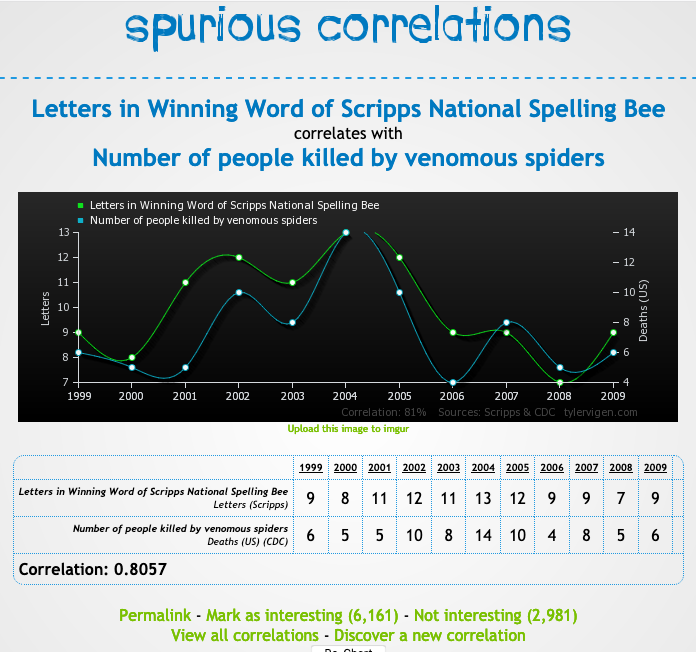
\includegraphics[width=.75\textheight]{graphics/spiders_spelling}
            }
        };
    \end{tikzpicture}

\href{https://www.tylervigen.com/spurious-correlations}{Tyler Vigen's Spurious Correlations}
\end{frame}

\begin{frame}
\frametitle{Why causality?}
\framesubtitle{To estimate effects of interventions}
\centering
\begin{tikzpicture}

    \node[inner sep=0pt] (med_caption) at (0,0) {

    };
    \node[inner sep=0pt, below=0.5cm of med_caption] (med)  {
        \fbox{
            
\includegraphics[width=.9\textheight]{graphics/mediterranean}
        }
    };

\end{tikzpicture}

\href{https://pubmed.ncbi.nlm.nih.gov/29897866/}{Article on PubMed}
\end{frame}

\begin{frame}{Interventions and causality}
    Ideal: Intervention + \href{https://en.wikipedia.org/wiki/Multiverse}{Multiverse} $\rightarrow$ Causality\newline

    Examples:
    \begin{itemize}
        \item Medical treatment (e.g. \href{https://en.wikipedia.org/wiki/Simpson\%27s_paradox\#Kidney_stone_treatment}{kidney stone treatment})
        \item Social outcomes (e.g. \href{https://en.wikipedia.org/wiki/Simpson\%27s_paradox\#UC_Berkeley_gender_bias}{university admissions})
        \item Business outcomes (e.g. \href{https://en.wikipedia.org/wiki/Click-through\_rate}{click-through rate}, hit rate)\newline
    \end{itemize}

    In-practice:
    \begin{itemize}
        \item Correlation: approximate multiverse by comparing intervention at $t$ to result at $t-1$
        \item Random population: approximate multiverse by splitting sample well
        \item A / B testing: random populations A / B + intervention in one
    \end{itemize}
\end{frame}


\begin{frame}{Formalizing interventions: the intuition of ``do" for hit-rate}
    For business application, quantity of interest is effect of intervention / counterfactual %$P(\textrm{hit}=1 | \textrm{days}=d)$, but intervention $$P(\textrm{hit}=1 | \jpdo(\textrm{days}=d))$$.\newline
    \begin{columns}[T] % align columns
        \begin{column}{.48\textwidth}
        Not $P(\textrm{hit}=1 | \textrm{days}=d)$\newline
        \begin{figure}[ht]
            $G = $ 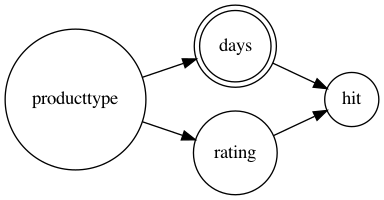
\includegraphics[height=0.55\textwidth]{graphics/given_days}
        \end{figure}
        \end{column}%
    %    \hfill%
        \begin{column}{.48\textwidth}
            but $P(\textrm{hit}=1 | \jpdo(\textrm{days}=d))$\newline
                \begin{figure}[ht]
                $G' = G_{\underline{\textrm{days}}} =$
                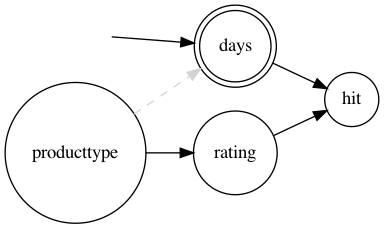
\includegraphics[height=0.55\textwidth]{graphics/do_days}
            \end{figure}
        \end{column}%
    \end{columns}
\end{frame}

\begin{frame}{Causality vs correlation mean different business decisions}
    Compute relative average treatment effect for different values of $\textrm{days}$:
    \begin{align*}
        \textrm{relative-ate}_G &= \frac{
            P_G(\textrm{hit}=1 | \textrm{days}=d) - P_G(\textrm{hit}=1 | \textrm{days}=d+1)
        }{P_G(\textrm{hit}=1 | \textrm{days}=d)} \\
        \textrm{relative-ate}_{G'} &= \frac{
            P_G(\textrm{hit}=1 | \jpdo(\textrm{days}=d)) - P_G(\textrm{hit}=1 | \jpdo(\textrm{days}=d+1))
        }{P_G(\textrm{hit}=1 | \jpdo(\textrm{days}=d))} \\
        & = \frac{
            P_{G'}(\textrm{hit}=1 | \textrm{days}=d) - P_{G'}(\textrm{hit}=1 | \textrm{days}=d+1)
        }{P_{G'}(\textrm{hit}=1 | \textrm{days}=d)}
    \end{align*}
    \begin{center}
        \begin{tabular}{rrrr}
\toprule
 from-d &  to-d &  ate-given &   ate-do \\
\midrule
      0 &     1 &   0.170153 & 0.297187 \\
      1 &     2 &   0.252329 & 0.395158 \\
      2 &     3 &   0.473538 & 0.102707 \\
\bottomrule
\end{tabular}

    \end{center}
\end{frame}


\begin{frame}
    \frametitle{Reality check and wrap-up}
    \begin{itemize}
        \item The \textrm{do}-calculus models interventions better than correlation / conditionals, but what about model misspecification?
        \item Causal reasoning mitigates risk of outsourcing thinking to correlations
    \end{itemize}
\end{frame}

\begin{frame}
    \frametitle{Appendices}
    For more context and code samples, see the \href{https://github.com/munichpavel/risk-ai-workshop/}{risk-ai-workshop repo} and \href{https://github.com/munichpavel/risk-ai-workshop/releases/tag/v2022.1.2}{slides}.
\end{frame}

\begin{frame}
\frametitle{Formalizing interventions: the intuition of ``do"}
	First, find quantities unchanged between $G$ and $G' = G_{\underline{\textrm{days}}}$
         \begin{figure}[ht]
             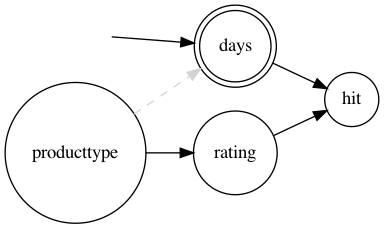
\includegraphics[height=0.5\textheight]{graphics/do_days}
        \end{figure}
        \vspace{-0.5cm}
        \begin{align}
        P_{G'}( & \textrm{producttype} = p, \textrm{rating} = r) \nonumber \\
        & = P_G( \textrm{producttype} = p, \textrm{rating} = r) \\
        P_{G'}(&\textrm{hit}=1 | \textrm{producttype} = p, \textrm{rating} = r) \nonumber  \\
        & = P_G(\textrm{hit}=1 | \textrm{producttype} = p, \textrm{rating} = r)
        \end{align}
\end{frame}


\begin{frame}{Formalizing interventions: the intuition of ``do"}
    \vspace{-1.5cm}
    \begin{tikzpicture}
        \node[] (q_0) at (0, 0) { };
        \node[] (q_1) [right=9cm of q_0]{
            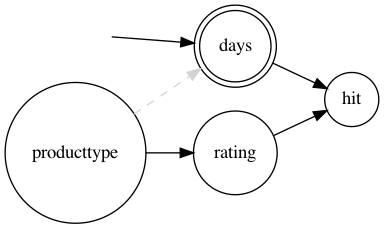
\includegraphics[width=.35\textwidth]{graphics/do_days}
        };
    \end{tikzpicture}
    \vspace{-2.5cm}
    \begin{align*}
        P(&\textrm{hit}=1 | \jpdo(\textrm{days})=d) \\
        & = P_{G'}(\textrm{hit}=1 | \textrm{days}=d) \textrm{, by definition} \\
        & = \sum_{p, r} P_{G'}(\textrm{hit}=1 | \textrm{days}=d, \textrm{producttype} = p, \textrm{rating} = r) \\
        & \qquad  \qquad P_{G'}(\textrm{producttype} = p, \textrm{rating} = r | \textrm{days}=d)\textrm{, by total probability} \\
        & = \sum_{p, r} P_{G'}(\textrm{hit}=1 | \textrm{days}=d, \textrm{producttype} = p, \textrm{rating} = r) \\
        & \qquad  \qquad P_{G'}(\textrm{producttype} = p, \textrm{rating} = r), \textrm{ by substitution} \\
        & =  \sum_{p, r} P_{G}(\textrm{hit}=1 | \textrm{days}=d, \textrm{producttype} = p, \textrm{rating} = r) \\
        & \qquad  \qquad P_{G}(\textrm{producttype} = p, \textrm{rating} = r), \textrm{ our \emph{adjustment} formula}
    \end{align*}
    References: \href{http://bayes.cs.ucla.edu/PRIMER/}{Judea Pearl et. al, Causal Inference in Statistics}, \href{https://cprohm.de/article/causality-and-function-approximations.html/}{Christopher Prohm, Causality and Function Approximation}
\end{frame}


\begin{frame}{Judea Pearl's Rules of Causality}

    Let $X$, $Y$ , $Z$ and $W$ be arbitrary disjoint sets of nodes in a DAG $G$. Let $G_\underline{X}$ be the graph obtained by removing all arrows pointing into (nodes of) $X$.
    Denote by $G_{\overline{X}}$ the graph obtained by removing all arrows pointing out of $X$. If, e.g. we remove arrows pointing out of $X$ and into $Z$, we the resulting graph is denoted by $G_{\underline{X} \overline{Z}}$

    Rule 1: Insertion / deletion of observations
    \begin{equation*}
        P(y | \jpdo(x), z, w) = P(y | \jpdo(x), w) \textrm{ if } (Y \ci Z | X, W)_{G_{\overline{X}}}
    \end{equation*}

    Rule 2: Action / observation exchange
    \begin{equation*}
        P(y | \jpdo(x), \jpdo(z), w) = P(y | \jpdo(x), z, w) \textrm{ if } (Y \ci Z | X, W)_{G_{\overline{X} \underline{Z}}}
    \end{equation*}

    Rule 3: Insertion / deletion of actions
    \begin{equation*}
        P(y | \jpdo(x), \jpdo(z), w) = P(y | \jpdo(x), w) \textrm{ if } (Y \ci Z | X, W)_{G_{\overline{X} \overline{Z(W)}}},
    \end{equation*}

    where $Z(W)$ is the set of $Z$-nodes that are not ancestors of any $W$-node in $G_\underline{X}$.

\end{frame}


\begin{frame}{Special cases of the causal rules}

    By judicious setting of sets of nodes to be empty, we obtain some useful corollaries of the causal rules.
    \newline

    Rule 1': Insertion / deletion of observations, with $W = \emptyset$
    \begin{equation*}
        P(y | \jpdo(x), z) = P(y | \jpdo(x)) \textrm{ if } (Y \ci Z | X)_{G_{\overline{X}}}
    \end{equation*}

    Rule 2': Action / observation exchange, with $X = \emptyset$
    \begin{equation*}
        P(y | \jpdo(z), w) = P(y | z, w) \textrm{ if } (Y \ci Z | W)_{G_{ \underline{Z}}}
    \end{equation*}

    Rule 3': Insertion / deletion of actions, with $X, W = \emptyset$
    \begin{equation*}
        P(y | \jpdo(z)) = P(y) \textrm{ if } (Y \ci Z )_{G_{\overline{Z}}}
    \end{equation*}

    \onslide<2->\textcolor{blue}{$\implies$ d-separation + causal rules = \emph{adjustment formulas}: $\jpdo$ queries as normal queries.}
\end{frame}

\begin{frame}{Causality vs correlation mean different business decisions}
    Quantity of interest: \emph{average treatment effect} or \emph{ATE}
    \begin{columns}[T] % align columns
        \begin{column}{.48\textwidth}
            $P(\textrm{hit}=1 | \textrm{days}=d)$\newline

            \input{graphics/given_days}\newline\newline
        \end{column}%
        \begin{column}{.48\textwidth}
            $P(\textrm{hit}=1 | \jpdo(\textrm{days}=d))$\newline

            \input{graphics/do_days}\newline \newline
        \end{column}%
    \end{columns}
\end{frame}

\end{document}